%\documentclass[9pt]{scrartcl}
\documentclass[a4paper]{article}
\usepackage[]{amsmath}
\usepackage{tikz}
\usetikzlibrary{positioning}
%\usepackage{helvet}
\usepackage{listings}
\usepackage{geometry}
%\geometry{textheight=\paperheight, noheadfoot, nomarginpar}
\usetikzlibrary{positioning,shapes,shadows}
\renewcommand{\familydefault}{\sfdefault}

\tikzstyle{abstract}=[rectangle, draw=black, fill=gray!20, text centered,  text=black, text width=12.5mm]
\tikzstyle{spacestyle}=[rectangle, draw=black, fill=gray!20, text centered,  text=black, text width=50mm]

\lstset{
        language=python,
        basicstyle=\fontencoding{T1}\ttfamily,
        commentstyle=\color{gray},
        keywordstyle=\color{OliveGreen},
        frame=single,
        backgroundcolor=\color{lightlightgray},
        tabsize=2,
        %deletestring=[d]",
        %escapechar=\%,
        numbers=left,
        showstringspaces=false,
}
\usepackage[explicit]{titlesec} 
\titleformat{\section}{\normalfont\Large\bfseries}{}{0em}{#1}
\titleformat{\subsection}{\normalfont\bfseries}{}{0em}{--#1}

\newcommand{\mykey}[2]{%
\begin{tikzpicture} \node (Item) [abstract, minimum size=12.5mm, align=center]
{\vrule height 12pt depth 8pt width 0pt\textbf{#1} \\\vrule height 6pt depth 8pt width 0pt\parbox{1.25cm}{\centering{\fontsize{6pt}{8pt}\selectfont{#2}}}};%
\end{tikzpicture}}


\begin{document}
\begin{center}
\Large{Diagram}
\end{center}
\noindent%


\section {Architecture diagram}
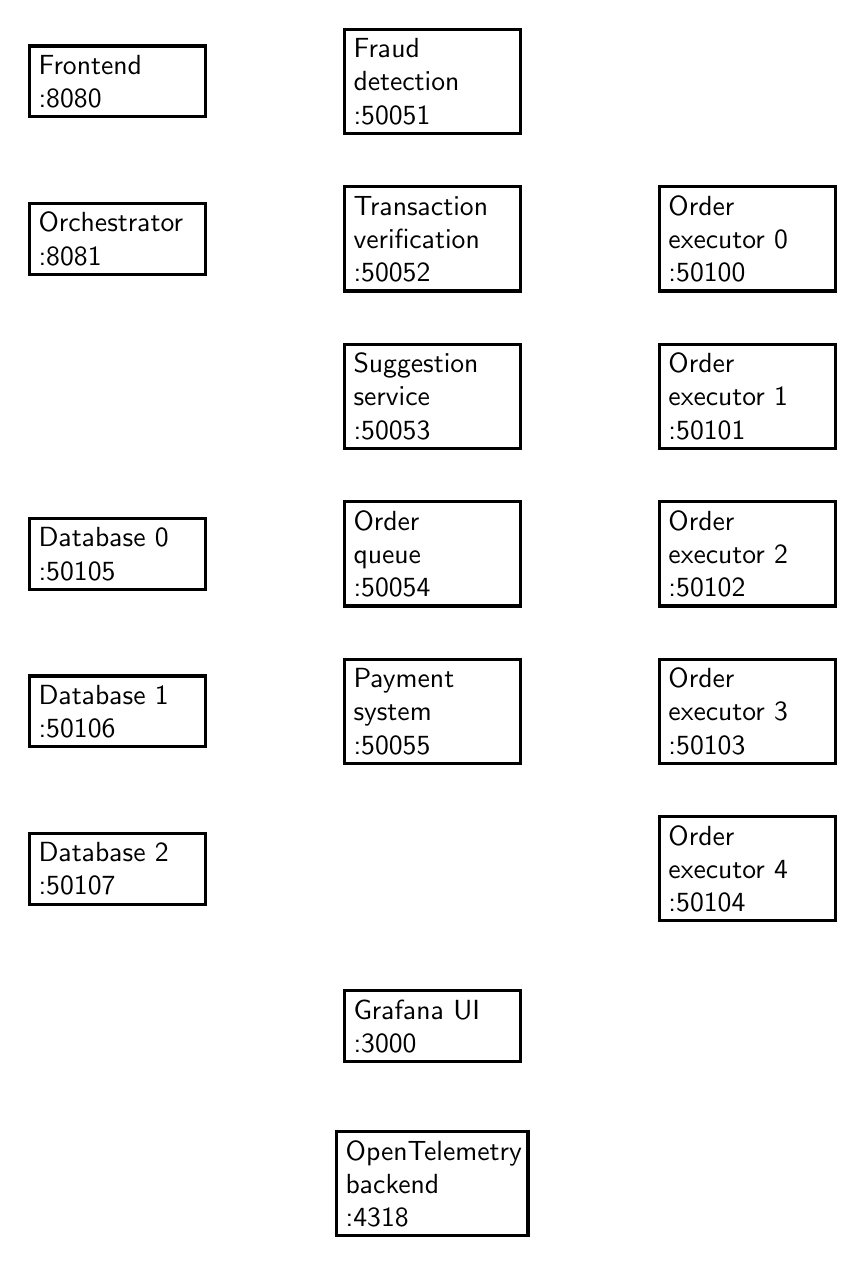
\begin{tikzpicture}

% Frontend
\node [draw,
	minimum width=2cm,
	text width=2cm,
	very thick,
]  (frontend) at (0, 0) {
Frontend\\
:8080
};

% Orchestrator
\node [draw,
	minimum width=2cm,
	text width=2cm,
	very thick
]  (orchestrator) at (0, -2) {
Orchestrator\\
:8081
};

% Fraud detection
\node [draw,
	minimum width=2cm,
	text width=2cm,
	very thick
]  (fraud_detection) at (4, 0) {
Fraud\\detection\\
:50051
};

% Transaction verifier
\node [draw,
	minimum width=2cm,
	text width=2cm,
	very thick
]  (transaction_verification) at (4, -2) {
Transaction\\verification\\
:50052
};

% Suggestions service
\node [draw,
	minimum width=2cm,
	text width=2cm,
	very thick
] (suggestions_service) at (4, -4) {
Suggestion\\service\\
:50053
};

% Order queue
\node [draw,
	minimum width=2cm,
	text width=2cm,
	very thick
] (order_queue) at (4, -6) {
Order\\queue\\
:50054
};

% Order executor 0
\node [draw,
	minimum width=2cm,
	text width=2cm,
	very thick
] (order_executor_0) at (8, -2) {
Order\\executor 0\\
:50100
};

% Order executor 1
\node [draw,
	minimum width=2cm,
	text width=2cm,
	very thick
] (order_executor_1) at (8, -4) {
Order\\executor 1\\
:50101
};

% Order executor 2
\node [draw,
	minimum width=2cm,
	text width=2cm,
	very thick
] (order_executor_2) at (8, -6) {
Order\\executor 2\\
:50102
};

% Order executor 3
\node [draw,
	minimum width=2cm,
	text width=2cm,
	very thick
] (order_executor_3) at (8, -8) {
Order\\executor 3\\
:50103
};

% Order executor 4
\node [draw,
	minimum width=2cm,
	text width=2cm,
	very thick
] (order_executor_4) at (8, -10) {
Order\\executor 4\\
:50104
};

% Database 0
\node [draw,
	minimum width=2cm,
	text width=2cm,
	very thick
] (database_0) at (0, -6) {
Database 0\\
:50105
};

% Database 1
\node [draw,
	minimum width=2cm,
	text width=2cm,
	very thick
] (database_1) at (0, -8) {
Database 1\\
:50106
};

% Database 2
\node [draw,
	minimum width=2cm,
	text width=2cm,
	very thick
] (database_2) at (0, -10) {
Database 2\\
:50107
};

% Payment system
\node [draw,
	minimum width=2cm,
	text width=2cm,
	very thick
] (payment_system) at (4, -8) {
Payment\\system\\
:50055
};

% Grafana UI
\node [draw,
	minimum width=2cm,
	text width=2cm,
	very thick
] (grafana_ui) at (4, -12) {
Grafana UI\\
:3000
};

% OpenTelemetry backend
\node [draw,
	minimum width=2cm,
	text width=2.2cm,
	very thick
] (opentelemetry_backend) at (4, -14) {
OpenTelemetry\\backend\\
:4318
};



% Arrows with text label

%\draw[thick] (frontend) -- (orchestrator) node[midway, right] {HTTP};
%\draw[thick] (orchestrator.east) -- (fraud_detection.west) node[midway, above] {RPC};
%\draw[thick] (orchestrator.east) -- (transaction_verification.west) node[midway, above] {RPC};
%\draw[thick] (orchestrator.east) -- (suggestions_service.west) node[midway, above] {RPC};

\end{tikzpicture}


\end{document}